\section{OpenCL}

\subsection{Language Overview}

Open Computing Language (OpenCL) is a framework for writing applications
designed to be executed across heterogeneous platforms such as central
processing units (CPUs), graphics processing units (GPUs), and accelerator
devices such as the Intel Xeon Phi and Field-Programmable Gate Arrays (FPGAs).
The language is an open standard maintained by Khronos Group
\footnote{\url{http://www.khronos.org/opencl}}. OpenCL is based on the C99
\footnote{\url{http://www.open-std.org/jtc1/sc22/wg14/www/docs/n1124.pdf}}
standard and can be loosely thought of as a subset of the C99 language with some
additional keywords. The first release of the OpenCL standard (OpenCL 1.0) was
on the 8th of December 2008. There have been two subsequent stable releases of
the standard, OpenCL 1.1 and 1.2, on the 14th of June 2010 and 15th of November
2011 respectively. The version with most hardware support is OpenCL 1.1
\footnote{\url{http://www.khronos.org/registry/cl/specs/opencl-1.1.pdf}} and
this standard forms the basis of all discussion on OpenCL in this report.

OpenCL splits the program code into two sections called `host' and `device'.
Host code runs on the CPU and is written in a traditional language such as C or
C++. The host code executes in the same way as a traditional application and
makes use of APIs exposed by OpenCL to define how, and where, OpenCL device code
is executed.

OpenCL applications are called kernels. A kernel is a function that executes on
an OpenCL capable device. Since the focus of OpenCL is on parallelism, a kernel
is written from the perspective of a single thread instead of requiring explicit
threading code from more familiar models such as POSIX threads. An OpenCL work
item is similar to a POSIX thread with a notable exception that OpenCL has no
traditional stack, any `function' calls by the OpenCL kernel are actually
in-lined by the compiler in some implementations. OpenCL kernels are also
compiled at runtime thus the host code, and the compiler itself, can make
device-specific optimisations for optimal performance.

\subsection{Models}

To accommodate the variety of devices OpenCL is designed to work with, a more
abstract memory model, and concurrency and execution model was designed to allow
the programmer full access to the target devices' capabilities. This complicates
the developer's job, by requiring them to think at a lower level of abstraction
than what they may be used to, however this is required to allow the application
to make the most out of the target hardware.

\subsubsection{Memory Model}

For a traditional C/C++ application, the application programmer can make use of
the primary memory space of the computer, typically DDR2 or DDR3 RAM. There are
caches on the CPU die however no direct control over their contents is offered.
For CPUs this is not an issue, all modern CPUs support automatic caching.
Problems occur when considering other devices, such as a GPU. GPUs do not
typically have automatic caching thus a programmer must make use of OpenCLs
abstract memory model, and hardware vendors must map this model to the physical
hardware. The OpenCL memory model defines four different types of memory, each
of which will be outlined below. A simplified diagrammatic representation of the
memory model is shown in Figure \ref{fig:openCLMemoryModel}.

\begin{description}

\item[Global memory] This memory is accessible by all compute units and is
similar to primary memory on a traditional CPU system. All work items are able
to access and update everything stored in this memory. For a GPU this is memory
mapped to the primary memory of the GPU and is typically 1-4GB in size. When
transferring data between the host's primary memory and the OpenCL device, this
is where the data has to reside. Global memory is denoted as `\_\_global' in an
OpenCL kernel.

\item[Constant memory] Constant memory resides in the same space as global
memory and is used for data which is accessed simultaneously by all work items,
or for variables whose values never change. Constant memory is denoted as
`\_\_constant' in an OpenCL kernel.

\item[Local memory] This is scratch pad memory which is only visible to a single
compute unit on the device. Local memory can be split up into distinct sections
if a single compute unit is executing multiple work- groups simultaneously.
Local memory is generally on- chip memory and thus has faster access time than
global memory. Local memory is typically on the order of tens of kilobytes in
size. Use of local memory is either statically declared in the kernel (e.g
`\_\_local float[64] localArray') or dynamically allocated at runtime by the
host. OpenCL kernels do not offer dynamic memory allocation during kernel
runtime.

Variables in local memory are not what would be called `local variables' in a
traditional application, OpenCL local variables are in private memory. Variables
in local memory are shared across a single work group, which can contain
multiple work items.

\item[Private memory] This is memory that is unique to an individual work item.
Any local variables and non-pointer kernel arguments are private by default.
These are typically mapped to registers although they can be spilled over to
higher latency memories if there is insufficient space available.

\end{description}

\begin{figure}
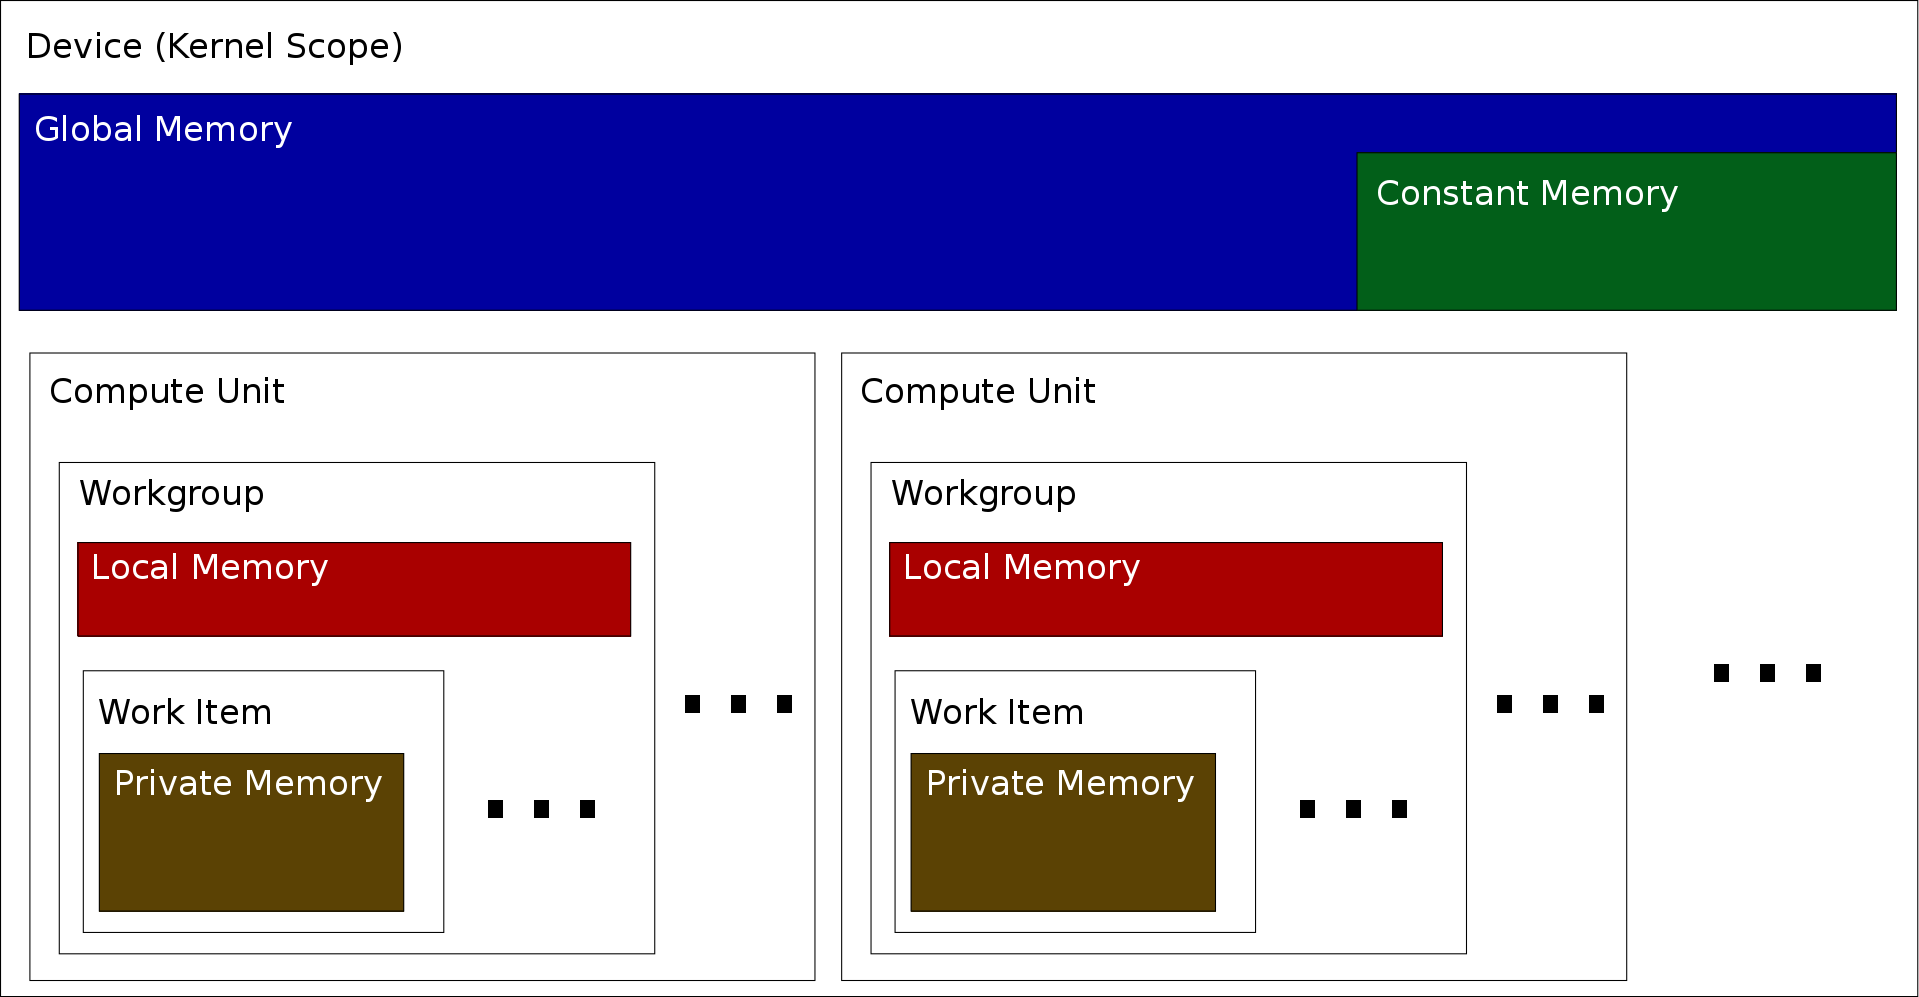
\includegraphics[width=\linewidth]{images/openCLMemoryModel.png}
\caption{Simplified visualisation of OpenCL Memory Model}
\label{fig:openCLMemoryModel}
\end{figure}

\subsubsection{Concurrency and Execution Model}

As shown in Figure \ref{fig:openCLMemoryModel}, OpenCL uses a number of
different terms to describe its execution model. There is no explicit `thread'
so instead OpenCL has work items which are the closest relative to traditional
threads. The OpenCL Concurrency and Execution Model is split into two parts,
host and device, and both will be outlined below.

\paragraph{Host}

\begin{description}

\item[Host program] As discussed previously, a host program is a traditional
program (written in C/C++ for instance) and is executed on a CPU. The host
program is responsible for managing the execution of kernels by creating and
setting up command queues for memory commands, kernel execution commands, and
synchronisation of commands.

\item[Context] The host program defines a context for the OpenCL devices. The
context will include the kernels to be executed, the available OpenCL devices,
and the memory objects used by kernels.

\item[NDRange] This stands for N-Dimensional Range and defines how work items
are organised. Work items can be arranged into one, two, or three dimensions.
This can be designed to increase performance and improve clarity of kernel code.
For instance, modifying a two dimensional matrix would warrant having a two
dimensional range as an this would be the most natural way to map work items to
matrix elements.

\item[Device Type] OpenCL places devices into three different classifications.
CPUs, GPUs, and Accelerators. An example accelerator device would be the Intel
Xeon Phi
\footnote{\url{http://www.intel.com/content/www/us/en/processors/xeon/xeon-phi-detail.html}}.

\end{description}

\paragraph{Device}

\begin{description}

\item[Compute Unit] This is a generic term used to describe a multiprocessor on
a GPU, or a core of a CPU. For some devices (such as a GPU) a compute unit will
have dedicated local memory, visible only to itself. A single compute unit can
be assigned multiple work groups.

\item[Kernel] As discussed previously, OpenCL code which runs on an OpenCL
device is known as a kernel. These are written from the perspective of a single
work item (thread).

\item[Work group] This is a collection of work items. An entire work group is
assigned to one compute unit. The work items that are associated with the work
group can share local memory and can synchronise with one another.

\item[Work item] This closely resembles a single thread. Each work item is
assigned a work group. Every work item can access local memory of its work
group and can access all global and constant memory. A work item will also
have private variables which may or may not fit inside private memory.

\item[Global size] This represents the total number of work items in each
dimension. The result of the multiplication of the global size in each dimension
is the total number of work items being executed for the corresponding kernel.

\item[Local size] This represents the total number of work items in each
dimension for a single work group. The global size for a dimension has to be an
integer multiple of the local size for that dimension for the work group size
to be valid. This is to ensure work groups can fit inside the global dimension
size evenly.

\end{description}

\begin{figure}
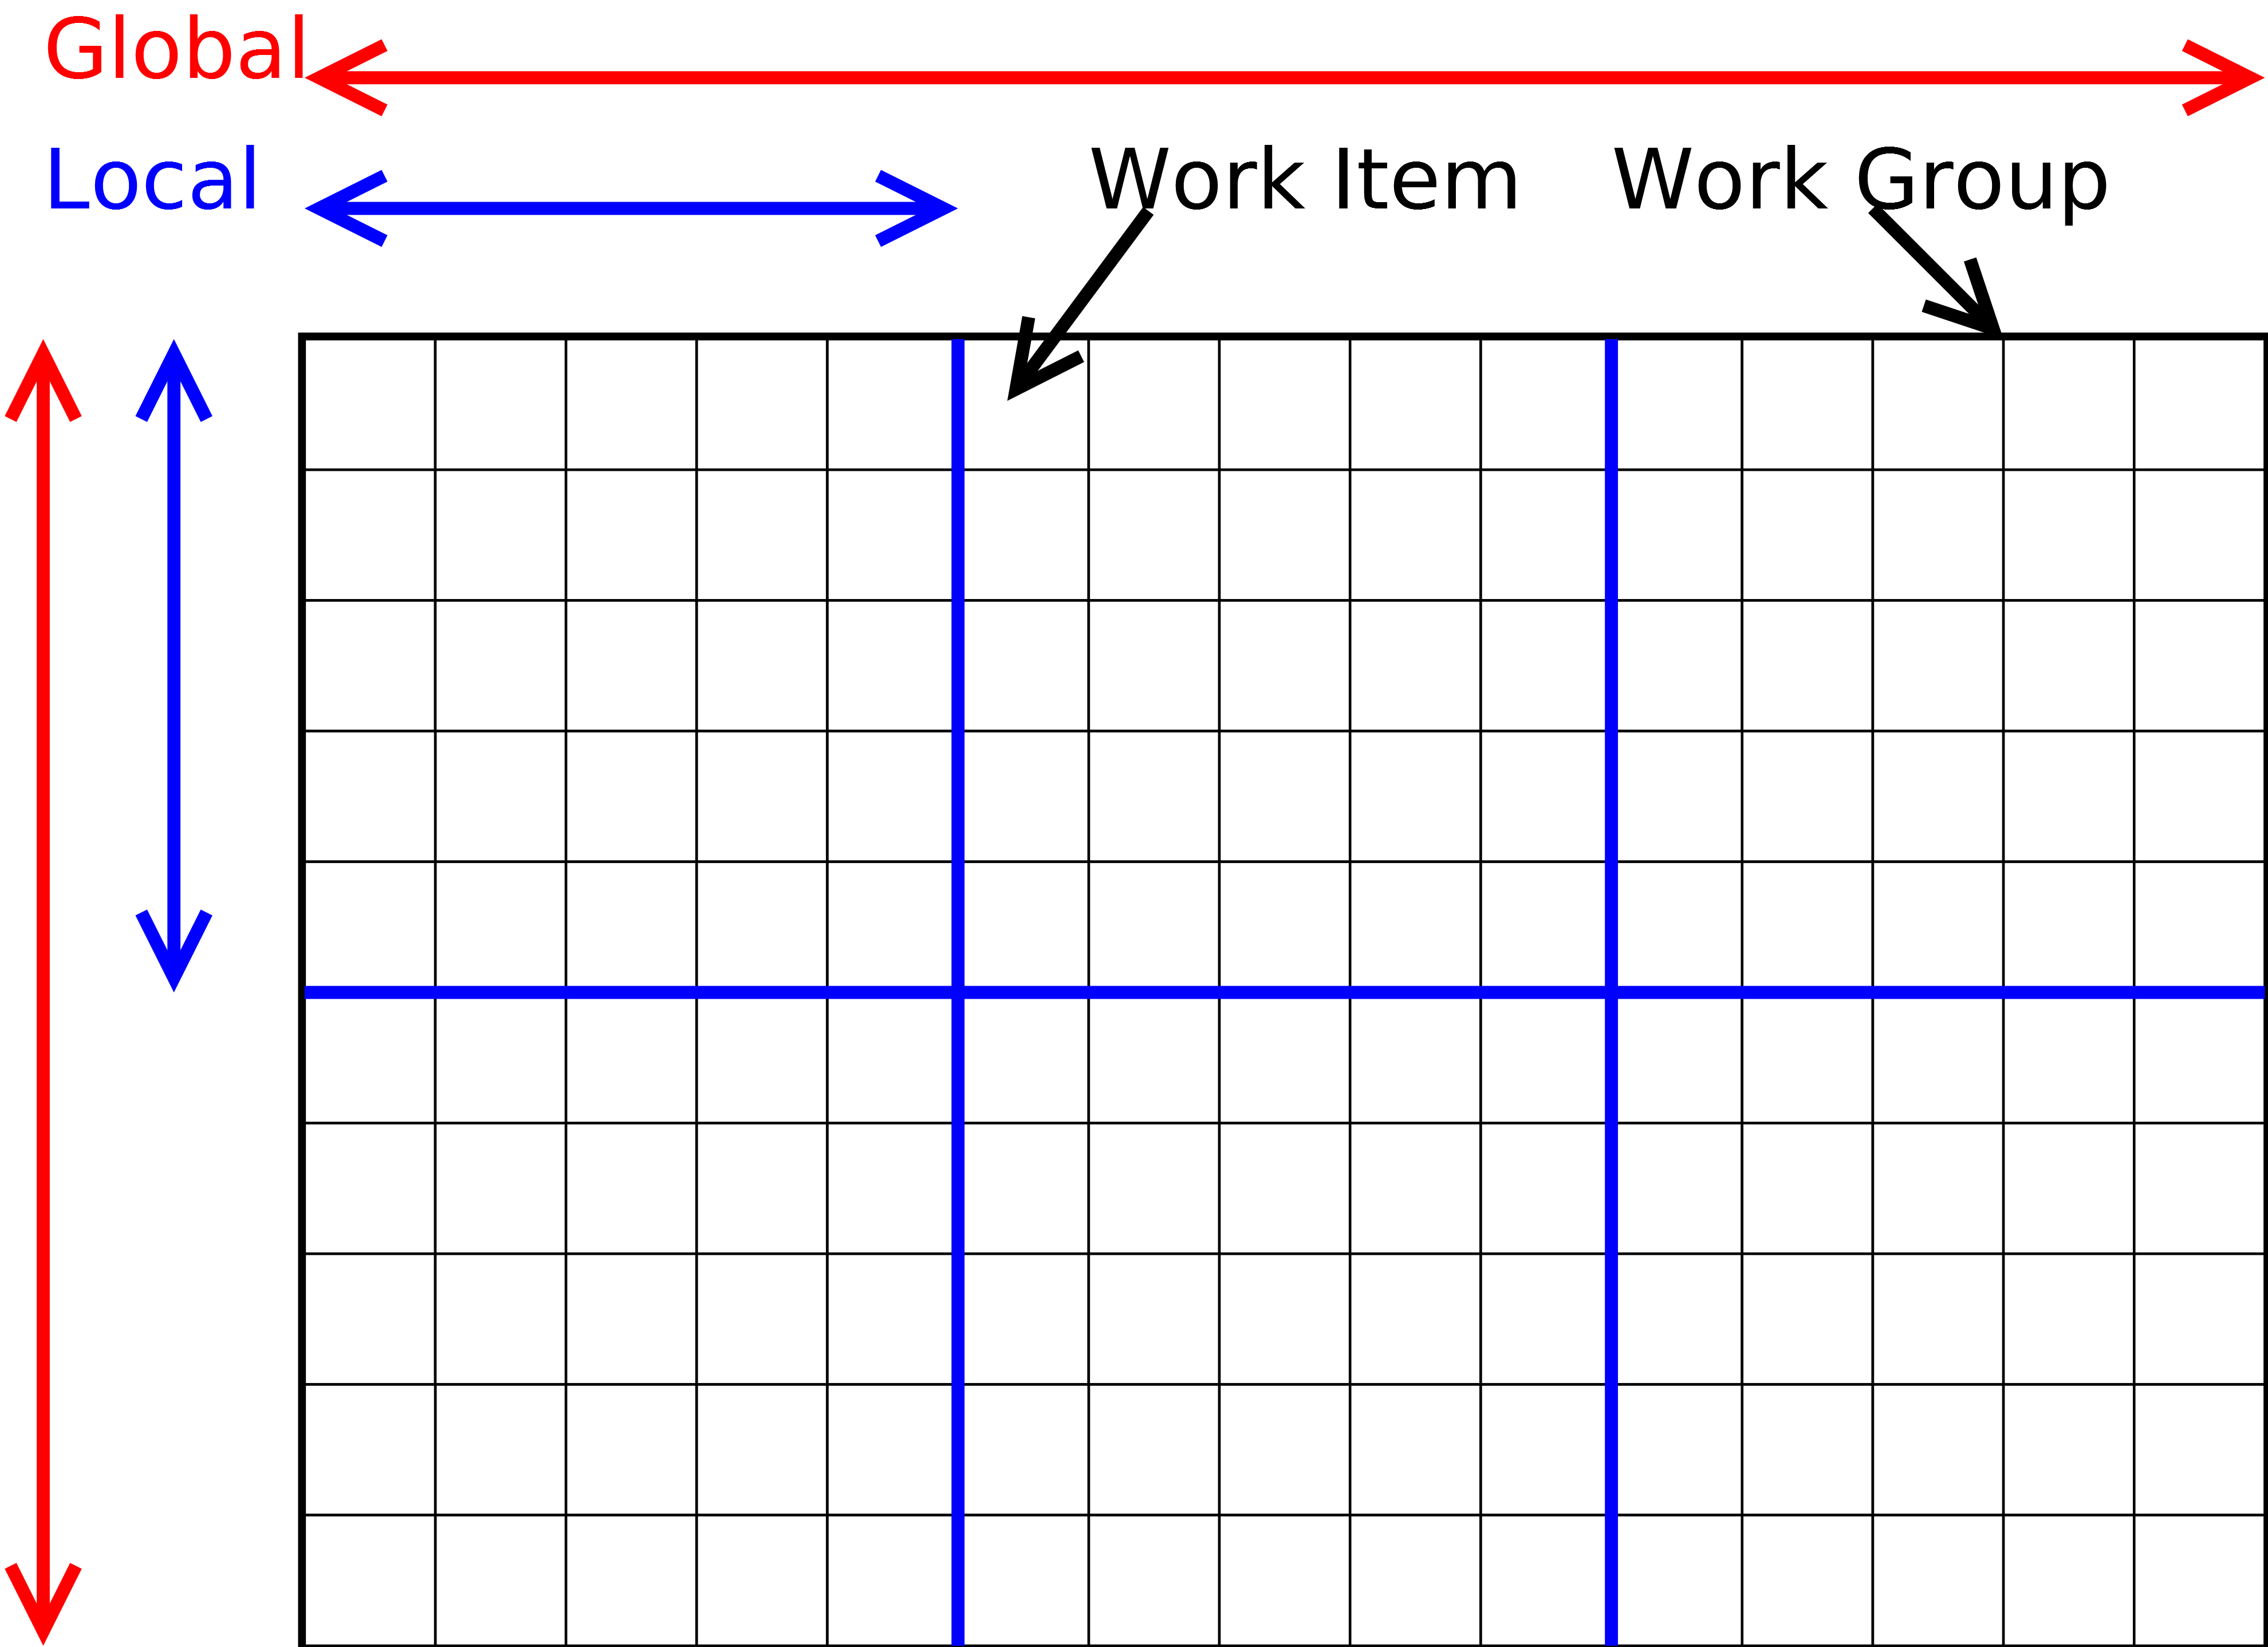
\includegraphics[width=\linewidth]{images/openCLExecutionModel.png}
\caption{Simplified visualisation of OpenCL Execution Model}
\label{fig:openCLExecutionModel}
\end{figure}

Figure \ref{fig:openCLExecutionModel} shows diagrammatically the relationship
between global and local size, and work items and work groups. Shown is a two
dimensional range, with global size of 15 for dimension 0, and 10 for dimension
1. Local size is 5 in both directions creating 6 work groups with 25 work items
each.

Just as with the Memory Model, different devices will realise the Concurrency
and Execution model differently. These differences will be discussed in the next
section.

\section{Device comparisons}

There are numerous important architecture differences between different classes
of device. At the high level, CPUs are aimed at being good all-rounders,
suitable for a multitude of tasks whereas GPUs have focused on the problem of
pixel value generation in a highly parallel fashion. This had led to the
evolution of different devices taking distinct paths. The important differences
will be outlined in this section.

\subsection{CPU and GPU}

The CPU is typically referred informally as the `brain' of the computer, not
only does it run the user's wide variety of software, it also acts as the
overall controller for the entire system. This necessitated a one-size-fits-all
style of approach when designing the CPU chip and the corresponding instruction
set architecture. A CPU typically has a high clock speed, in the range of 3-4GHz
for a modern desktop. Each die can contain a small number of cores, typically
four, that execute instructions simultaneously.

A GPU is the highly parallel oriented chip, with hundreds of cores running at a
slower clock speed (about one fifth of a CPU core) and with a more restricted
instruction set, primarily designed for simple, repetitive tasks needed for
video output.

\subsubsection{Threading and Cache}

A CPU has a few hardware threads, one or two per CPU core which occasional
context swtiching, with multi-level caching to reduce off-chip memory access
latency.

GPUs have many threads to keep compute units busy, if some threads are waiting
on memory accesses, other threads are available to run. Latency is thus hidden
rather than reduced. This has led to the design of a context switch for GPU
threads to have insignificant cost to help facilitate the latency hiding.

\subsubsection{Arithmetic Throughput}

GPUs use more of the transistor budget on arithmetic units than memory cache
compared to CPUs. This makes GPUs more suitable to high density arithmetic and
repetitive computations more than a CPU.

\subsubsection{Execution Model Implementation}

CPUs have a very free implementation of the OpenCL execution model. Threads are
free to take their own execution path, and aren't directly affected by other
thread's progress except from at explicit synchronisation stages.

GPUs, on the other hand, have a Single Instruction Multiple Threads (SIMT)
execution model. This means that GPUs have one instruction unit for multiple
arithmetic units. Threads are partitioned into groups which execute the same
instruction simultaneously. For nVidia GPUs these are referred to in the CUDA
model as `warps' and typically contain 32 threads. This can increase performance
as this reduces the number of fetch and decode operations on instructions
required. A performance consequence of this is in code with conditional
branches.

\begin{figure}[H]
\small\begin{verbatim}
if (someCondition)
{
    nonTrivialCode();
}
else
{
    someMoreNonTrivialCode();
}
\end{verbatim}
\end{figure}

For a simple example, consider the situation when someCondition is true for half
of the threads, and false for the other half of the threads. For a CPU each
thread executes the instructions by itself and some threads can be executing
`nonTrivialCode()' at the same time some threads are executing
`someMoreNonTrivalCode()'. However, on a GPU the threads in the true branch
execute their instructions while the other threads remain idle, and only after
the true branch has been completed, the false branch threads execute. This is
known as a divergent warp. Divergent warps can considerably reduce performance
as it reduces the number of threads executing in parallel and should be avoided
when developing an OpenCL kernel as much as possible.

In addition to instruction execution, memory accesses are done on a per warp
basis. For ideal performance, addressing should be such that threads in a warp
access coalesced memory locations to reduce memory transaction cost. For
instance, an array where access is based on a hash function can result in poor
performance as threads in a warp are likely to be accessing significantly
different parts of memory. If all threads access consecutive memory locations,
then one or two reads can be enough to supply data required by tens of threads,
rather than one read per thread.

\subsubsection{Extra performance consideration}

In addition to the architecture differences between CPUs and GPUs, there is a
separate consideration that must be made for GPUs and other discrete devices,
the PCIe bus. GPUs are unable to directly access main memory like a CPU, thus
before any code is run on a GPU, data must be transferred between primary memory
and the GPUs on-board memory. This can take a significant period of time in
comparison to the code runtime. This is due to the relatively slow speed of the
PCIe bus in comparison to on-board memory access. A GPU is able to access its
global memory at a rate of around 256GB/s on modern chips. Contrast this to the
PCIe link speed which can be as low as 250MB/s per lane. The most common systems
have PCIe 2.0 slots which run at 500MB/s per PCIe lane so, with 16 lanes
available for the GPU, this gives a maximum theoretical transfer speed of 8GB/s,
32 times slower than access from on-board memory.

\subsection{Bridging the gap - APUs}

Both CPUs and GPUs are strong in their respective application areas. Ideally, a
system should be able to make best use of both types of device with as little
overhead as possible. One of the obvious potential bottlenecks is the PCIe bus
to devices discrete from the CPU. This led to the design of an Accelerated
Processing Unit (APU). These have a traditional CPU in addition to a GPU (or
FPGA) on the same die and are a good example of a Heterogeneous System
Architecture (HSA). This design isn't new, CPUs have typically contained a small
GPU, especially in the small laptop market. With the growth of Heterogeneous
Systems, there has been a trend to increasing the GPU performance on die with
the CPU. This reduces the gap between the CPU and the GPU and removes the PCIe
bus overhead. The primary consumer implementation of this is AMDs HSA
\footnote{\url{http://developer.amd.com/resources/heterogeneous-computing/}}.
The joint die allows power to be managed so that different applications can make
most effective use of the CPU and GPU cycles available. In addition, there is
also work going on to completely unify address spaces, to make the heterogeneous
architecture more seamless to work with.

For the purposes of this report, APU discussion ends here. At present consumer
devices are relatively immature and for a majority of applications, a discrete
GPU or accelerator card is more likely to achieve the best overall performance.

\subsection{Intel Xeon Phi}

The Intel Xeon Phi is similar in many respects to a CPU, with around 60
x86-compatible CPU cores on a discrete card. The device additionally has 8GB of
on-board GDDR5 memory, similar to a GPU. The device sits in a PCIe slot like a
GPU and thus has the same performance considerations for the PCIe bus as a GPU.
A detailed look at the inner workings of the Intel Xeon Phi architecture can be
found on Intel's website
\footnote{\url{http://software.intel.com/en-us/articles/intel-xeon-phi-coprocessor-codename-knights-corner}}.

Each CPU core is on a bi-directional ring bus to memory and each core is capable
of 4-way hyper threading resulting in 240 hardware threads per device. Clock
speeds are typically lower than a CPU at around 1GHz. The Intel Xeon Phi is
designed to allow CPU-like programming versatility with the high performance and
efficient power use of an accelerator chip.

In addition to being an OpenCL capable device, the Xeon Phi is capable of
running applications written in traditional source code such as C, C++, or
FORTRAN. The device itself contains a Linux operating system which is
automatically started up and loads a file system, allows secure shell logins,
and enables a TCP/IP stack to facilitate communication as if the device was a
separate internal network device.

\subsubsection{Performance Considerations}

In addition to the PCIe bus consideration, the ring bus to memory needs to be
taken into consideration. This is most notable with communication between cores.
Communication between neighbouring cores will be fast, however communication
between cores on the `opposite side' of the ring will be significantly slower.

\section{Document Classification}

As discussed in Section~\ref{sec:relatedResearch} on related research, the work
in this report directly relates to and builds on work by Wim Vanderbauwhede et
al. The purpose of their work is to classify a stream of text documents based on
significant terms in the documents. A classic example would be emails, where
spam emails tend to have specific terms to indicate their class. An assumption
is that most of the documents will not be of interest (mostly not spam in our
example) so the profiles of significant terms discriminates highly. This is
achieved by a Na{\"{\i}}ve Bayes classifier with n-grams, similar to the work by
the University of Waterloo \cite{peng2003combining} for text classification and
Greek \cite{metsis2006spam} and German \cite{Schneider:2003:CEM:1067807.1067848}
academics for spam filtering itself.

The most recent papers by Wim Vanderbauwhede et al. discuss the use of FPGAs for
high throughput document filtering. The inherent parallelism in document
classification (as is also true with many data-centric algorithms) and the
parallelism focus of FPGAs, was found to be a suitable pairing to create a power
efficient, high throughput scoring system for parsed documents
\cite{vanderbauwhede2013high} \cite{HybridCPUFPGA}. The results of the latest
paper show that, while an FPGA can score at a median performance of 749MB/s
\cite{vanderbauwhede2013high}, the CPU can only parse at 426.2MB/s making the
parsing on the CPU the bottleneck to higher performance. This report will take
the same initial steps, implementing the scoring on a GPU, and then, due to the
parser being the bottleneck to performance, look into having parsing and scoring
on the GPU and other devices. This is similar to the work by Altera Toronto
Technology Center which focuses on performance per watt ratios
\cite{chen2012invited} but use manufacturer quoted board figures for power
usage, rather than measuring energy used from the power socket.

\subsection{Parser}

\subsubsection{Structure}

The parser is a Finite State Machine originally implemented in C++ but designed
to also be suitable for FPGA implementation. The parser is able to make full use
of all hardware threads available to it from the CPUs \cite{HybridCPUFPGA}. The
output from the parser is a series of terms (English language words) in a sixty
four bit number. Each term can contain up to twelve characters, with each
character being represented by five bits. The last four bits of the term are
used to identify the number of characters in the term. If a term is larger than
twelve characters, the remainder of the word is truncated. Given the average
English word length of 8.23 characters \footnote{\url{http://www.ravi.io
/language-word-lengths}} this is an acceptable encoding.

\subsubsection{Baudot Encoding}

The encoding used to convert an eight bit ASCII character into five bits is a
variant of Baudot encoding
\footnote{\url{http://rabbit.eng.miami.edu/info/baudot.html}}. Most text
compression algorithms are lossless, the original text can always be returned
during a decompression stage. Baudot code is different, it is lossy. The
compressed text can still be read as English, just with some character
substitutions. The algorithm is outlined in Figure~\ref{baudotCode}:

\begin{figure}[H]
\small\begin{verbatim}
to5BitEncoding(char c)
{
    if (c == 'i' || c == 'j' || c == 'I' || c == 'J')
    {
        return 1;
    }
    if (c == 'o' || c == 'O')
    {
        return 0;
    }
    if (isLowercase(c))
    {
        tcode = c - ((v > 106) ? ((v > 111) ? ((v > 117) ? 4 : 3) : 2) : 0);
        return tcode - 87;
    }
    if (isUpperCase(c))
    {
        tcode = c - ((v > 74) ? ((v > 79) ? ((v > 86) ? 4 : 3) : 2) : 0);
        return tcode - 55;
    }
    if (isNumeric(c))
    {
        return c - 48;
    }
}
\end{verbatim}
\caption{ASCII to 5 bit encoding pseudo code}
\label{baudotCode}
\end{figure}

In short, characters which look like a 1 (`i', `j', `I', and `J') are converted
to 1. Characters which look like a 0 (`o', `O') are converted to 0. `u', `v',
`U', and `V' are treated to be `U'. All other characters have their ASCII value
reduced so that they fit into numbers lower than 32. All lower case characters
are now upper case meaning now, in total, there are 10 (numeric) + 26 (letters)
- 4 (`I', `J', `O', and `V') = 32 characters.

\subsection{Scorer}

The array of terms is passed onto the scorer, prior this report this could be
another CPU routine, or an FPGA. The beginning of documents is marked by a term
representing the document ID. The last four bits (term length field) are left
at 0 to indicate that this is a document start.

\subsubsection{Terms and N-Grams}

Each term is taken in turn. N-grams (up to tri-grams) are created with the new
term. An n-gram is essentially a concatenation of the newest term onto the end
of the last n-1 terms, up to an n-gram length of twelve as with the original
terms. The reason behind this is that an English word on its own right isn't
always significant but with the previous words to place it in context, it may
be. A simple example from the area of spam filtering is the word `Rolex'. On its
own it's not necessarily important whereas with the tri-gram `Cheap Real Rolex',
it becomes more significant and indicates that the document in question is
likely spam.

\subsubsection{Profile}

After the n-grams have been generated, each one is taken in turn and looked up
in the profile of terms. The profile is a hashed data structure of (term,
weight) pairs. If the term exists in the profile, the weight of the term is
added to the document's score. It is this score which is ultimately used to
determine a document's classification. If the score is above a certain threshold
value, the document is significant to us, otherwise it isn't.

A profile is typically quite large, 128MB in this case. As such, the profile is
organised in such a way that it is a hashed array allowing for O(1) (constant
time) lookup rather than a linear, or binary search which would be O(n) and
O(log n) time respectively (where n is the number of elements in the profile).
To work out where a term is in the profile, a simple bit shift and masking
operation is executed to obtain an offset into the profile array. This allows
for the possibility of collisions with other terms thus probing is used (up to
four addresses) to reduce the likelihood of missing a term in the profile.

\subsubsection{Bloom Filters}

With the profile being large, it will always be mostly resident in main memory.
For the CPU system this is off chip, and for GPUs and accelerator devices this
is on the same board, but both have significantly higher latency than caches
which reside closer to the CPU cores and GPU compute units. With the profile
only containing a subset of possible terms, and the requirement to look up four
terms due to hashing collisions, the latency to go to main memory can end up
being quite significant. To reduce the need to go to main memory, a small data
structure (4KB or so) is employed called a bloom filter. Burton Bloom first
defined this data structure in a famous paper: ``Space/Time Trade-offs in Hash
Coding with Allowable Errors'' \cite{bloom1970space}.

A Bloom filter is used to store the possibility that a term exists in the
profile. With the size of the Bloom filter being small, it's likely it will
migrate into a cache of both the CPU and GPU allowing for efficient lookup of
the bloom filter and minimised trips to memory for non-existent profile terms.

A Bloom filter works as follows. It is an array of bit values where 0 indicates
absent and 1 indicates present. When constructing the profile, each entry is
run through a number of hash functions (for example, four) to get a number of
numerical values. These numerical values are indices for bit positions in the
bloom filter. These bit positions are set to 1.

To use the bloom filter, the term to be looked up is run through the same hash
functions. If all locations returned by the hash functions have their bit set to
1, then it's likely the term is in the profile. Even if n-1 out of n positions
are set to 1, with the nth set to 0, the profile is known not to contain the
term. However, it is possible that a term can have all n bit positions set to 1
but still be absent from the profile. Think of the case where term 1 sets
positions a, b, c, and d, and term 2 sets positions c, d, e, and f. An absent
term 3 could hash to positions b, c, d, and e which, although they are set to 1,
aren't contained in the profile. In other words, a bloom filter cannot have a
false negative result (all terms in profile can be looked up) but can have false
positive results like term 3.

This is the space/time tradeoff that Bloom discusses. A Bloom filter can be
very small compared to the data structure it's supporting but lookups can take
more time due to the false positive results. If the false positive rate is low
enough, the time saved from the reads from memory avoided by true negatives
outweighs the time wasted looking up false positive results.
